%\documentclass[11pt]{book}
%\usepackage{palatino}
%\usepackage{amsfonts,amsmath,amssymb}
%% \usepackage{graphicx}
%
%\usepackage{listings}
%\usepackage{textcomp}
%\usepackage{color}
%
%\definecolor{dkgreen}{rgb}{0,0.6,0}
%\definecolor{gray}{rgb}{0.5,0.5,0.5}
%\definecolor{mauve}{rgb}{0.58,0,0.82}
%
%\lstset{frame=tb,
%  language=R,
%  aboveskip=3mm,
%  belowskip=3mm,
%  showstringspaces=false,
%  columns=flexible,
%  basicstyle={\small\ttfamily},
%  numbers=none,
%  numberstyle=\tiny\color{gray},
%  keywordstyle=\color{blue},
%  commentstyle=\color{dkgreen},
%  stringstyle=\color{mauve},
%  breaklines=true,
%  breakatwhitespace=true,
%  tabsize=3
%}
%
%
%
%\ifx\pdftexversion\undefined
%    \usepackage[dvips]{graphicx}
%\else
%    \usepackage[pdftex]{graphicx}
%    \usepackage{epstopdf}
%    \epstopdfsetup{suffix=}
%\fi
%
%\usepackage{subfig}
%
%\begin{document}
%
%%%%%%%%%%%%%%%%%%%%%%%%%%%%%%%%%%%%%%%%%
%% Problem Set 3
%%%%%%%%%%%%%%%%%%%%%%%%%%%%%%%%%%%%%%%%%
%
%\pagestyle{empty}
%{\noindent\bf Spring 2023 \hfill Brandon~Parmanand}
%\vskip 16pt
%\centerline{\bf University of Central Florida}
%\centerline{\bf College of Business}
%\vskip 16pt
%\centerline{\bf QMB 6911}
%\centerline{\bf Capstone Project in Business Analytics}
%\vskip 10pt
%\centerline{\bf Solutions:  Problem Set \#3}
%\vskip 32pt
%\noindent
%
%\pagebreak
\section*{Normality of the Original and Transformed Variables}

Figure \ref{fig:qq_prices} shows a pair of Q-Q plots.
In the left panel, Figure \ref{subfig:qq_prices} shows this comparison 
for the original level of the house prices, without transformation. 
This figure shows that it deviates from the normal distribution.
In the right panel, Figure \ref{subfig:qq_log_prices} shows this comparison 
for the logarithmic transformation of house prices, without transformation. 
This figure also shows that it deviates from the normal distribution even though it is closer to it than the original level of the house prices.


\begin{figure}[!ht]
\subfloat[House Prices\label{subfig:qq_prices}]{%
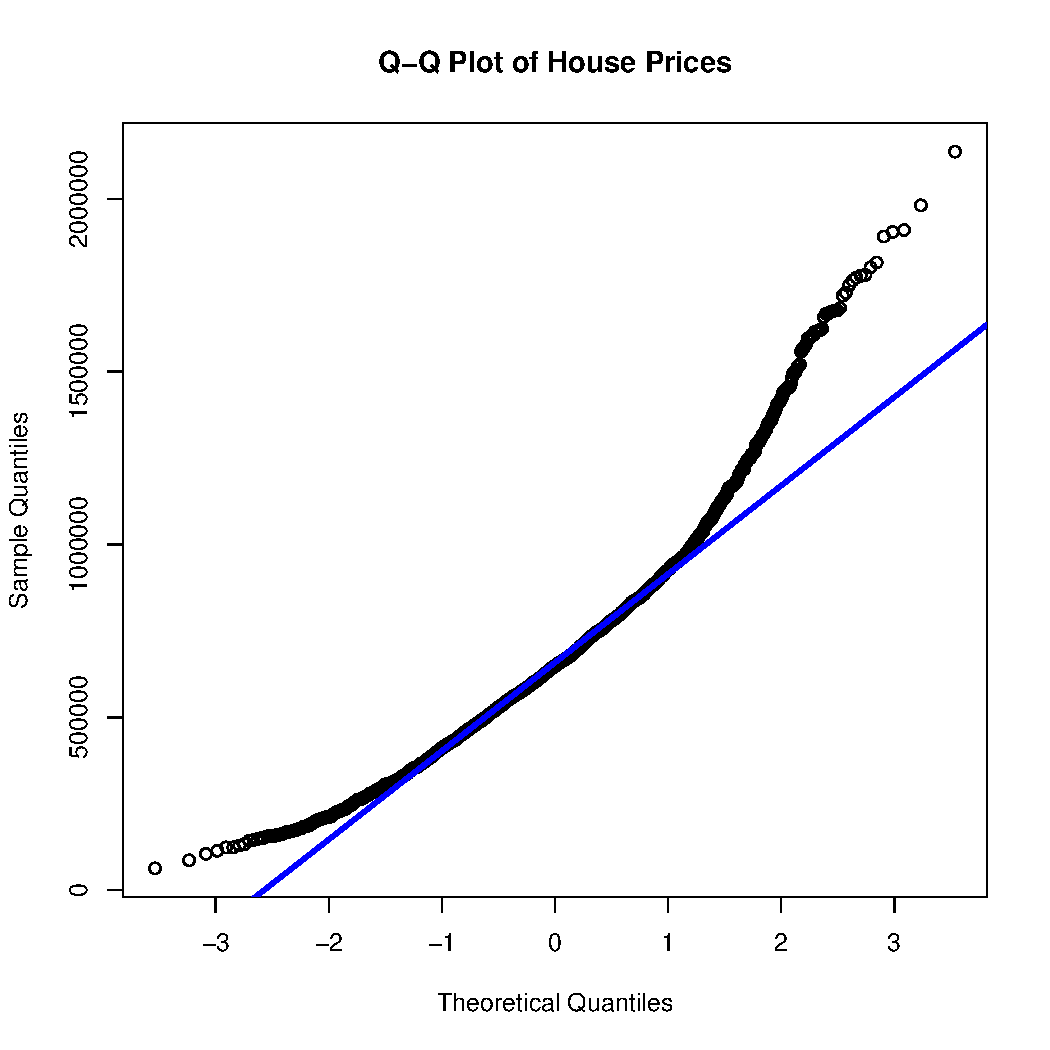
\includegraphics[width=0.5\textwidth]{../Figures/qq_prices}}
\hfill
\subfloat[Transformed House Prices\label{subfig:qq_log_prices}]{%
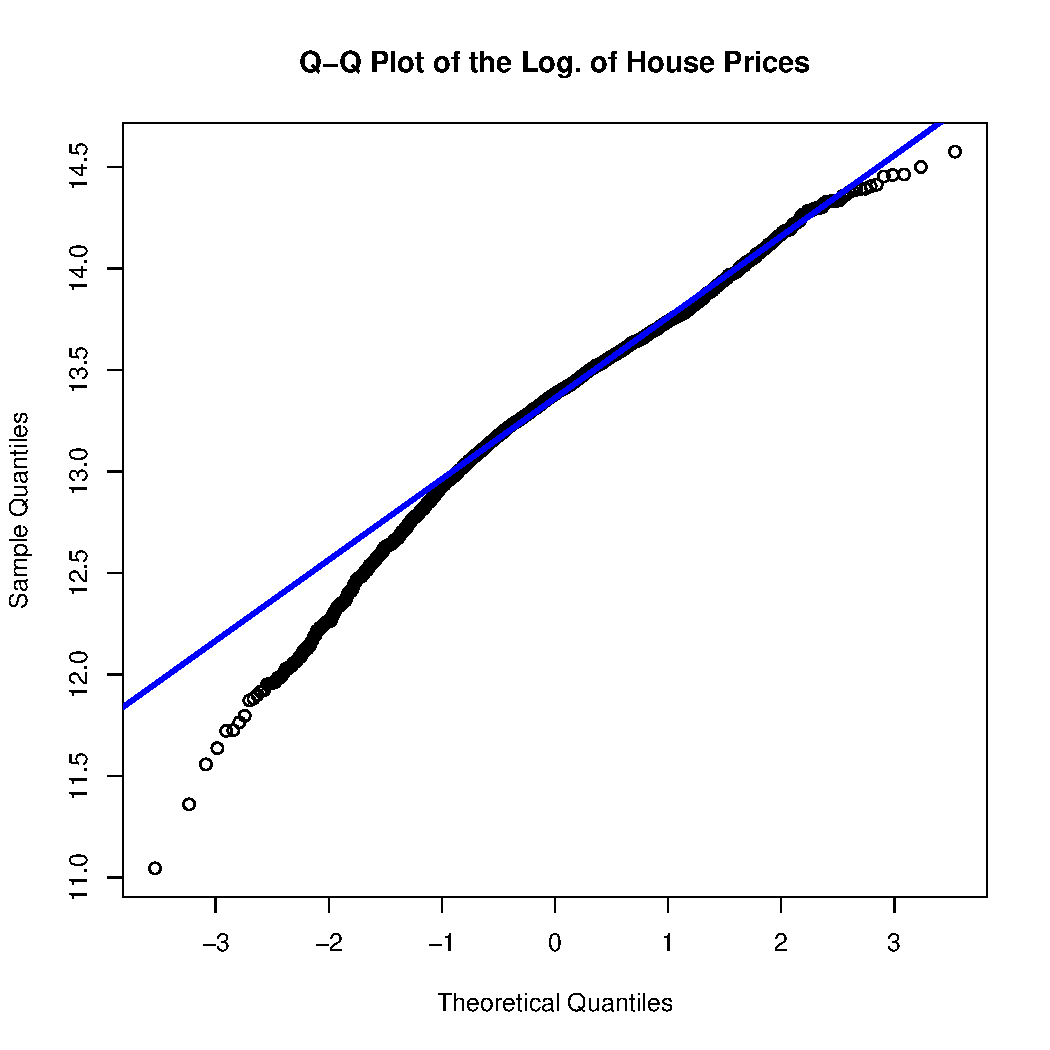
\includegraphics[width=0.5\textwidth]{../Figures/qq_log_prices}}

\caption{Q-QPlots of the Log. and Levels of House Prices}
\label{fig:qq_prices}
\end{figure}



%%%%%%%%%%%%%%%%%%%%%%%%%%%%%%%%%%%%%%%%
% Box-Cox Transformation
%%%%%%%%%%%%%%%%%%%%%%%%%%%%%%%%%%%%%%%%


\pagebreak
\section*{Box-Cox Transformation of House Prices}

The plot of this likelihood function is shown in Figure \ref{fig:box_cox_loglike_uni}.
The red points represent the values of the log-likelihood 
at the optimum $\lambda = 0.38$ and at $\lambda = 0$ and $\lambda = 1$.

\begin{figure}[h!]
  \centering
  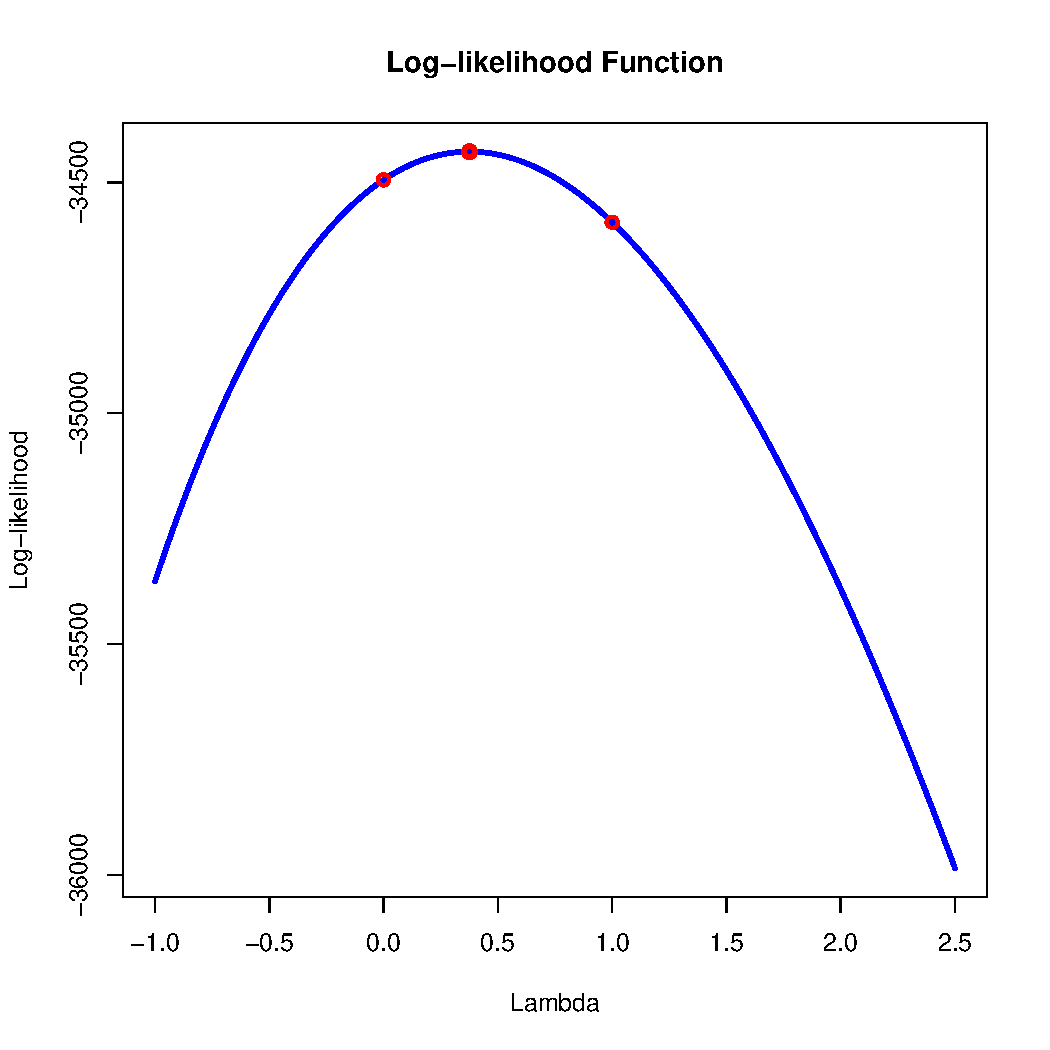
\includegraphics[scale = 0.5, keepaspectratio=true]{../Figures/box_cox_loglike_uni}
  \caption{Log-likelihood Function for Box-Cox Transformation} \label{fig:box_cox_loglike_uni}
\end{figure}


\pagebreak
\section*{Testing for an Appropriate Transformation using Likelihood Ratio}

Considering the statistical properties of these estimates
by calculating a likelihood ratio statistic. After doing the tests, 
we end up with a p-value of 0 for each so this is evidence to reject 
both and not transform with the linear or logarithmic specification.
This suggests using the transformation at the MLE but this will further 
complicate the statistical model.


\section*{Normality of the Transformed Variable}

Figure \ref{fig:qq_prices2} shows this comparison
and the panel on the right, Figure \ref{subfig:qq_boxcox}, 
shows that the quantiles of the distribution of the transformed variable
are much closer to the normal distribution but there is still a slightly notable deviation 
at $\lambda = 0.38$
Transforming at $\lambda = 0$ or $\lambda = 1$ 
was not done as the statistical test allowed us to reject those models.%
This provides statistical evidence that the prices are best modeled with the transformation
at the optimal $\lambda = 0.38$.
If other variables are added, the complexity of doing this may prove it to be not useful.


\begin{figure}[!ht]
\subfloat[Fly Reel Prices\label{subfig:qq_prices2}]{%
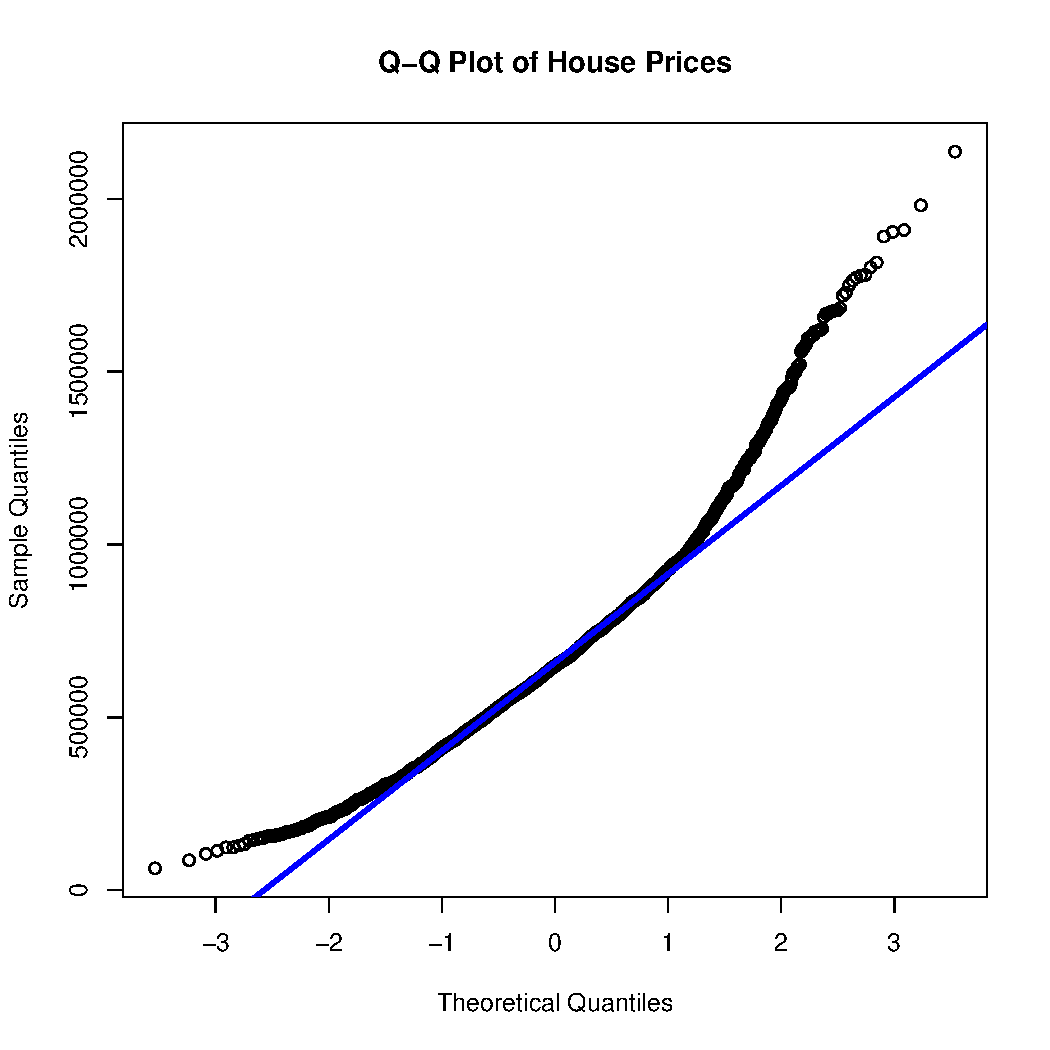
\includegraphics[width=0.5\textwidth]{../Figures/qq_prices2}}
\hfill
\subfloat[Transformed Fly Reel Prices\label{subfig:qq_boxcox}]{%
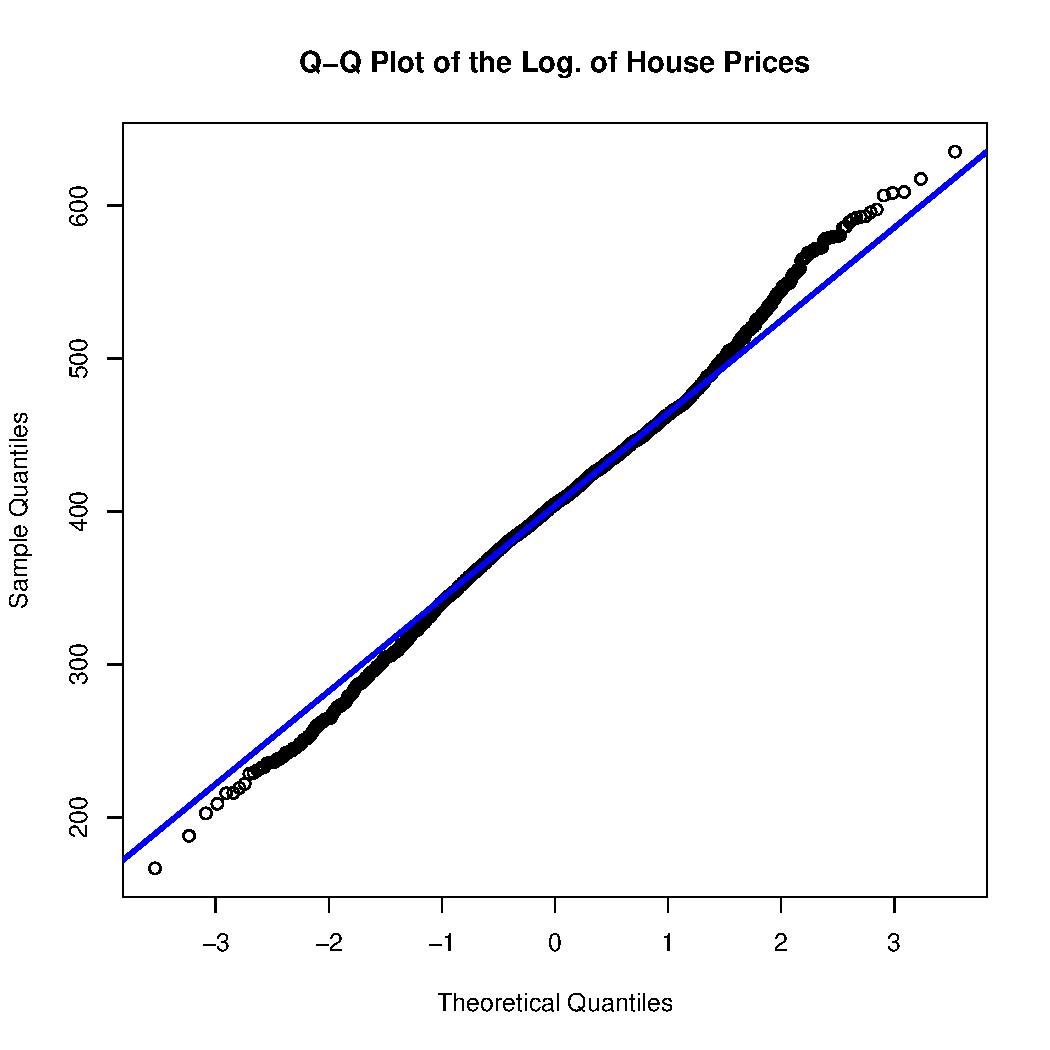
\includegraphics[width=0.5\textwidth]{../Figures/qq_boxcox}}

\caption{Q-QPlots of the Transformed Fly Reel Prices}
\label{fig:qq_prices2}
\end{figure}


\clearpage
\begin{figure}[!ht]
\subfloat[{Log. of House Prices}\label{subfig:qq_prices3}]{%
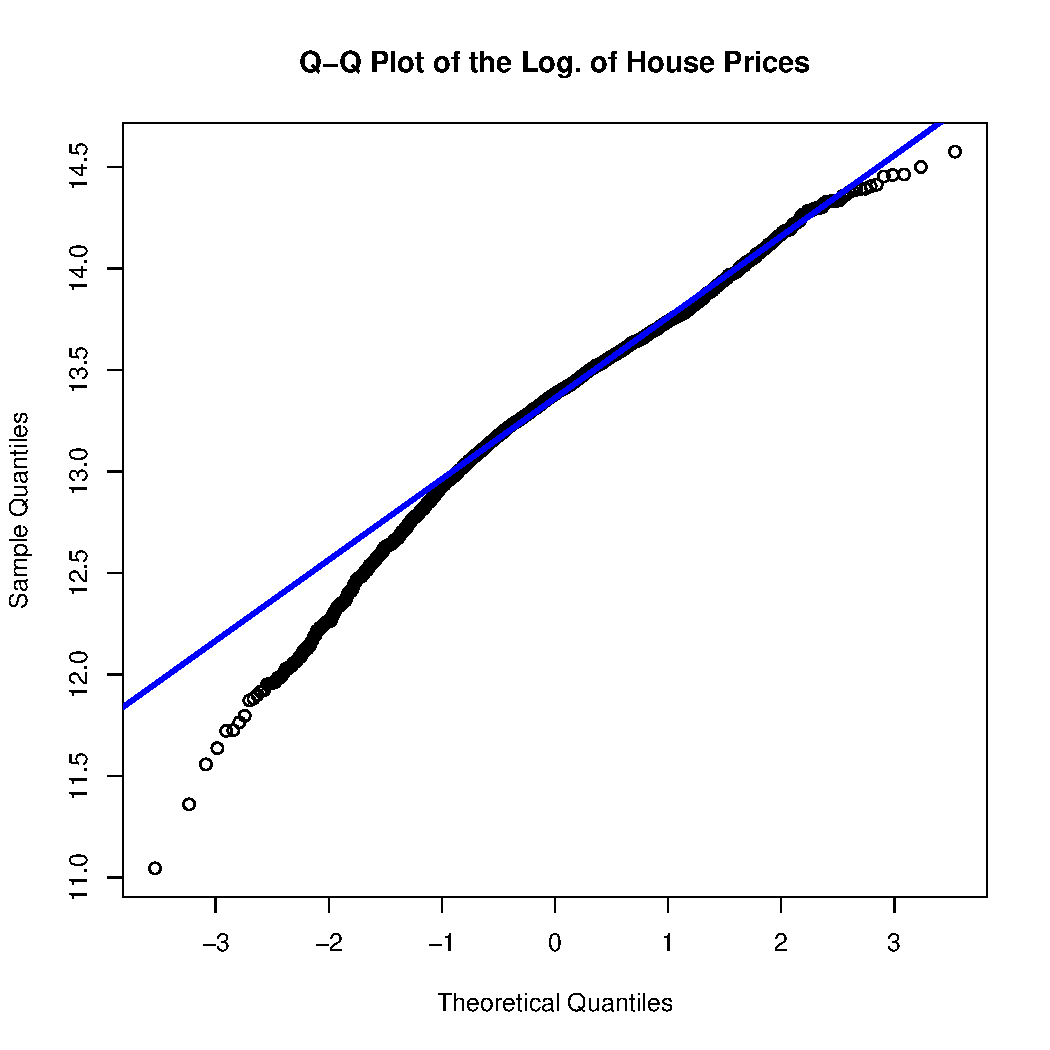
\includegraphics[width=0.5\textwidth]{../Figures/qq_log_prices}}
\hfill
\subfloat[Transformed House Prices\label{subfig:qq_boxcox_3}]{%
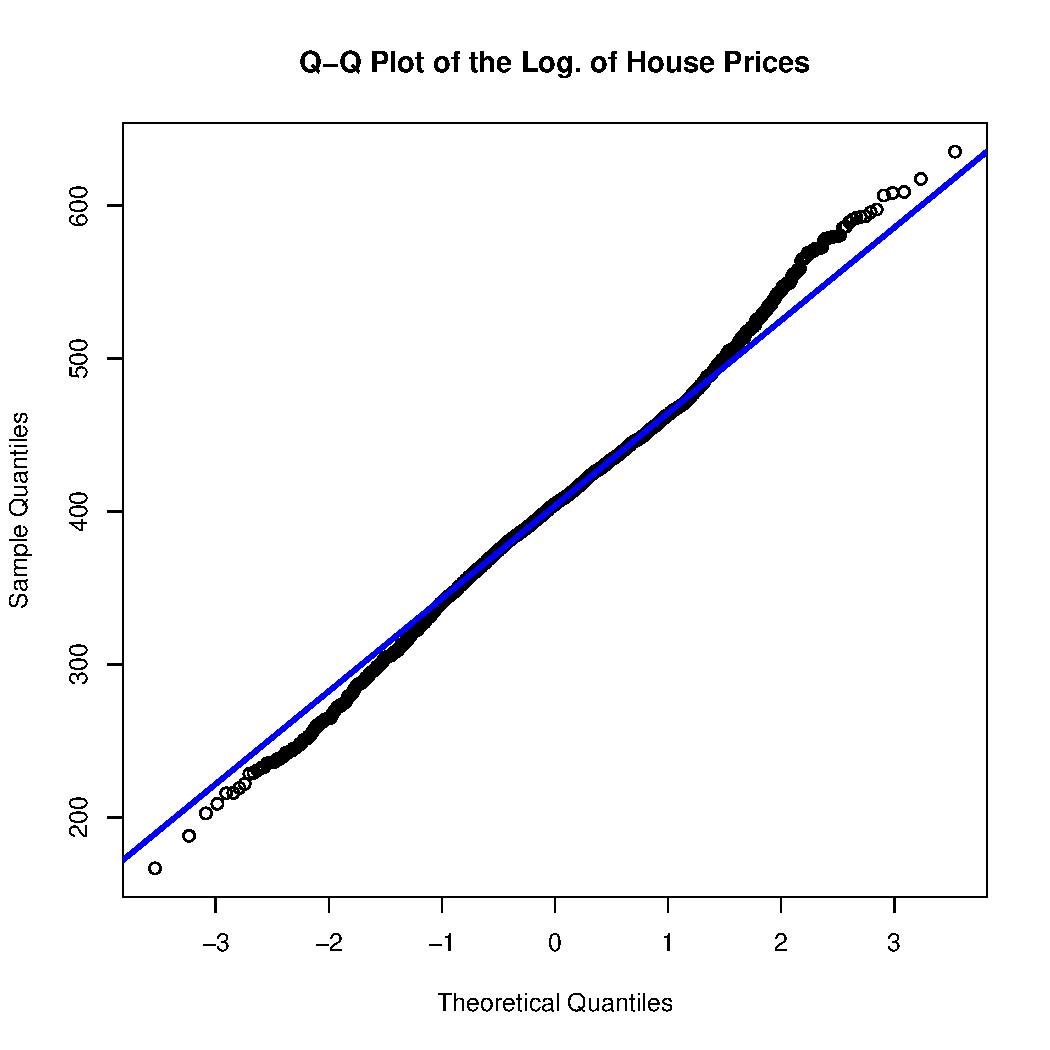
\includegraphics[width=0.5\textwidth]{../Figures/qq_boxcox}}

\caption{Q-QPlots of the Transformed House Prices}
\label{fig:qq_prices2}
\end{figure}


\clearpage

\section*{\textsf{R}  \texttt{MASS} Package for the Box-Cox Transformation}


I used the function from the \texttt{MASS} package to further my analysis.
The output is plotted in Figure \ref{fig:plot_like_MASS}. Figure \ref{subfig:plot_like_MASS_var}, 
shows that optimum is getting closer to 0 so even with the explanatory variables added%
we should take the logarithm of the prices. We get $\lambda = 0.33$ compared to 0.38 with the intial 
Box-Cox transformation. With all this info, I would not change my recommendation.
\begin{figure}[!ht]
\subfloat[ House Prices MASS\label{subfig:plot_like_MASS}]{%
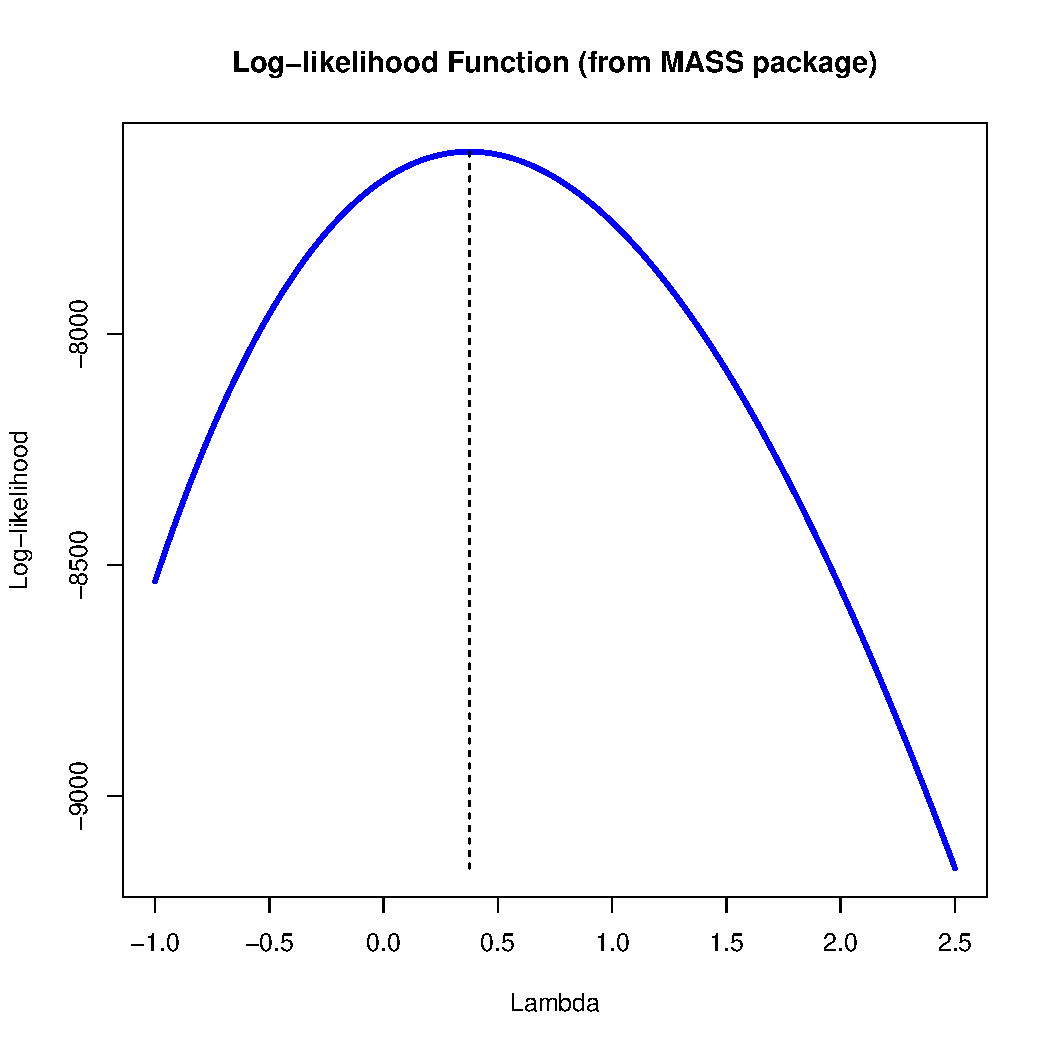
\includegraphics[width=0.5\textwidth]{../Figures/plot_like_MASS}}
\hfill
\subfloat[House Prices MASS with Vars\label{subfig:plot_like_MASS_var}]{%
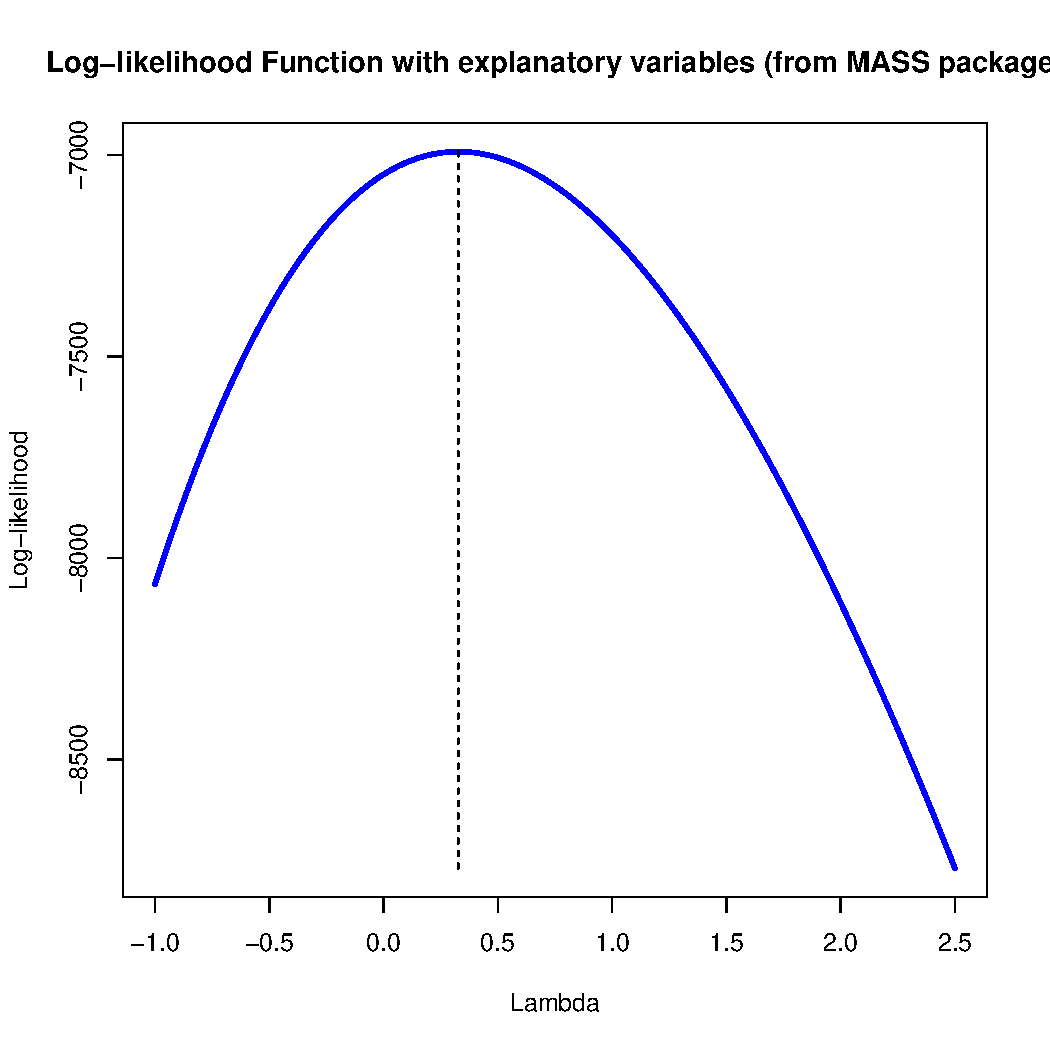
\includegraphics[width=0.5\textwidth]{../Figures/plot_like_MASS_var}}

\caption{ Transformed House Prices}
\label{fig:plot_like_MASS}
\end{figure}










%%%%%%%%%%%%%%%%%%%%%%%%%%%%%%%%%%%%%%%%
%\end{document}
%%%%%%%%%%%%%%%%%%%%%%%%%%%%%%%%%%%%%%%%
